Voici ci-dessous, la structure originale de la machine au commencement de ce projet de Bachelor :
\begin{figure}[H]
  \centering
  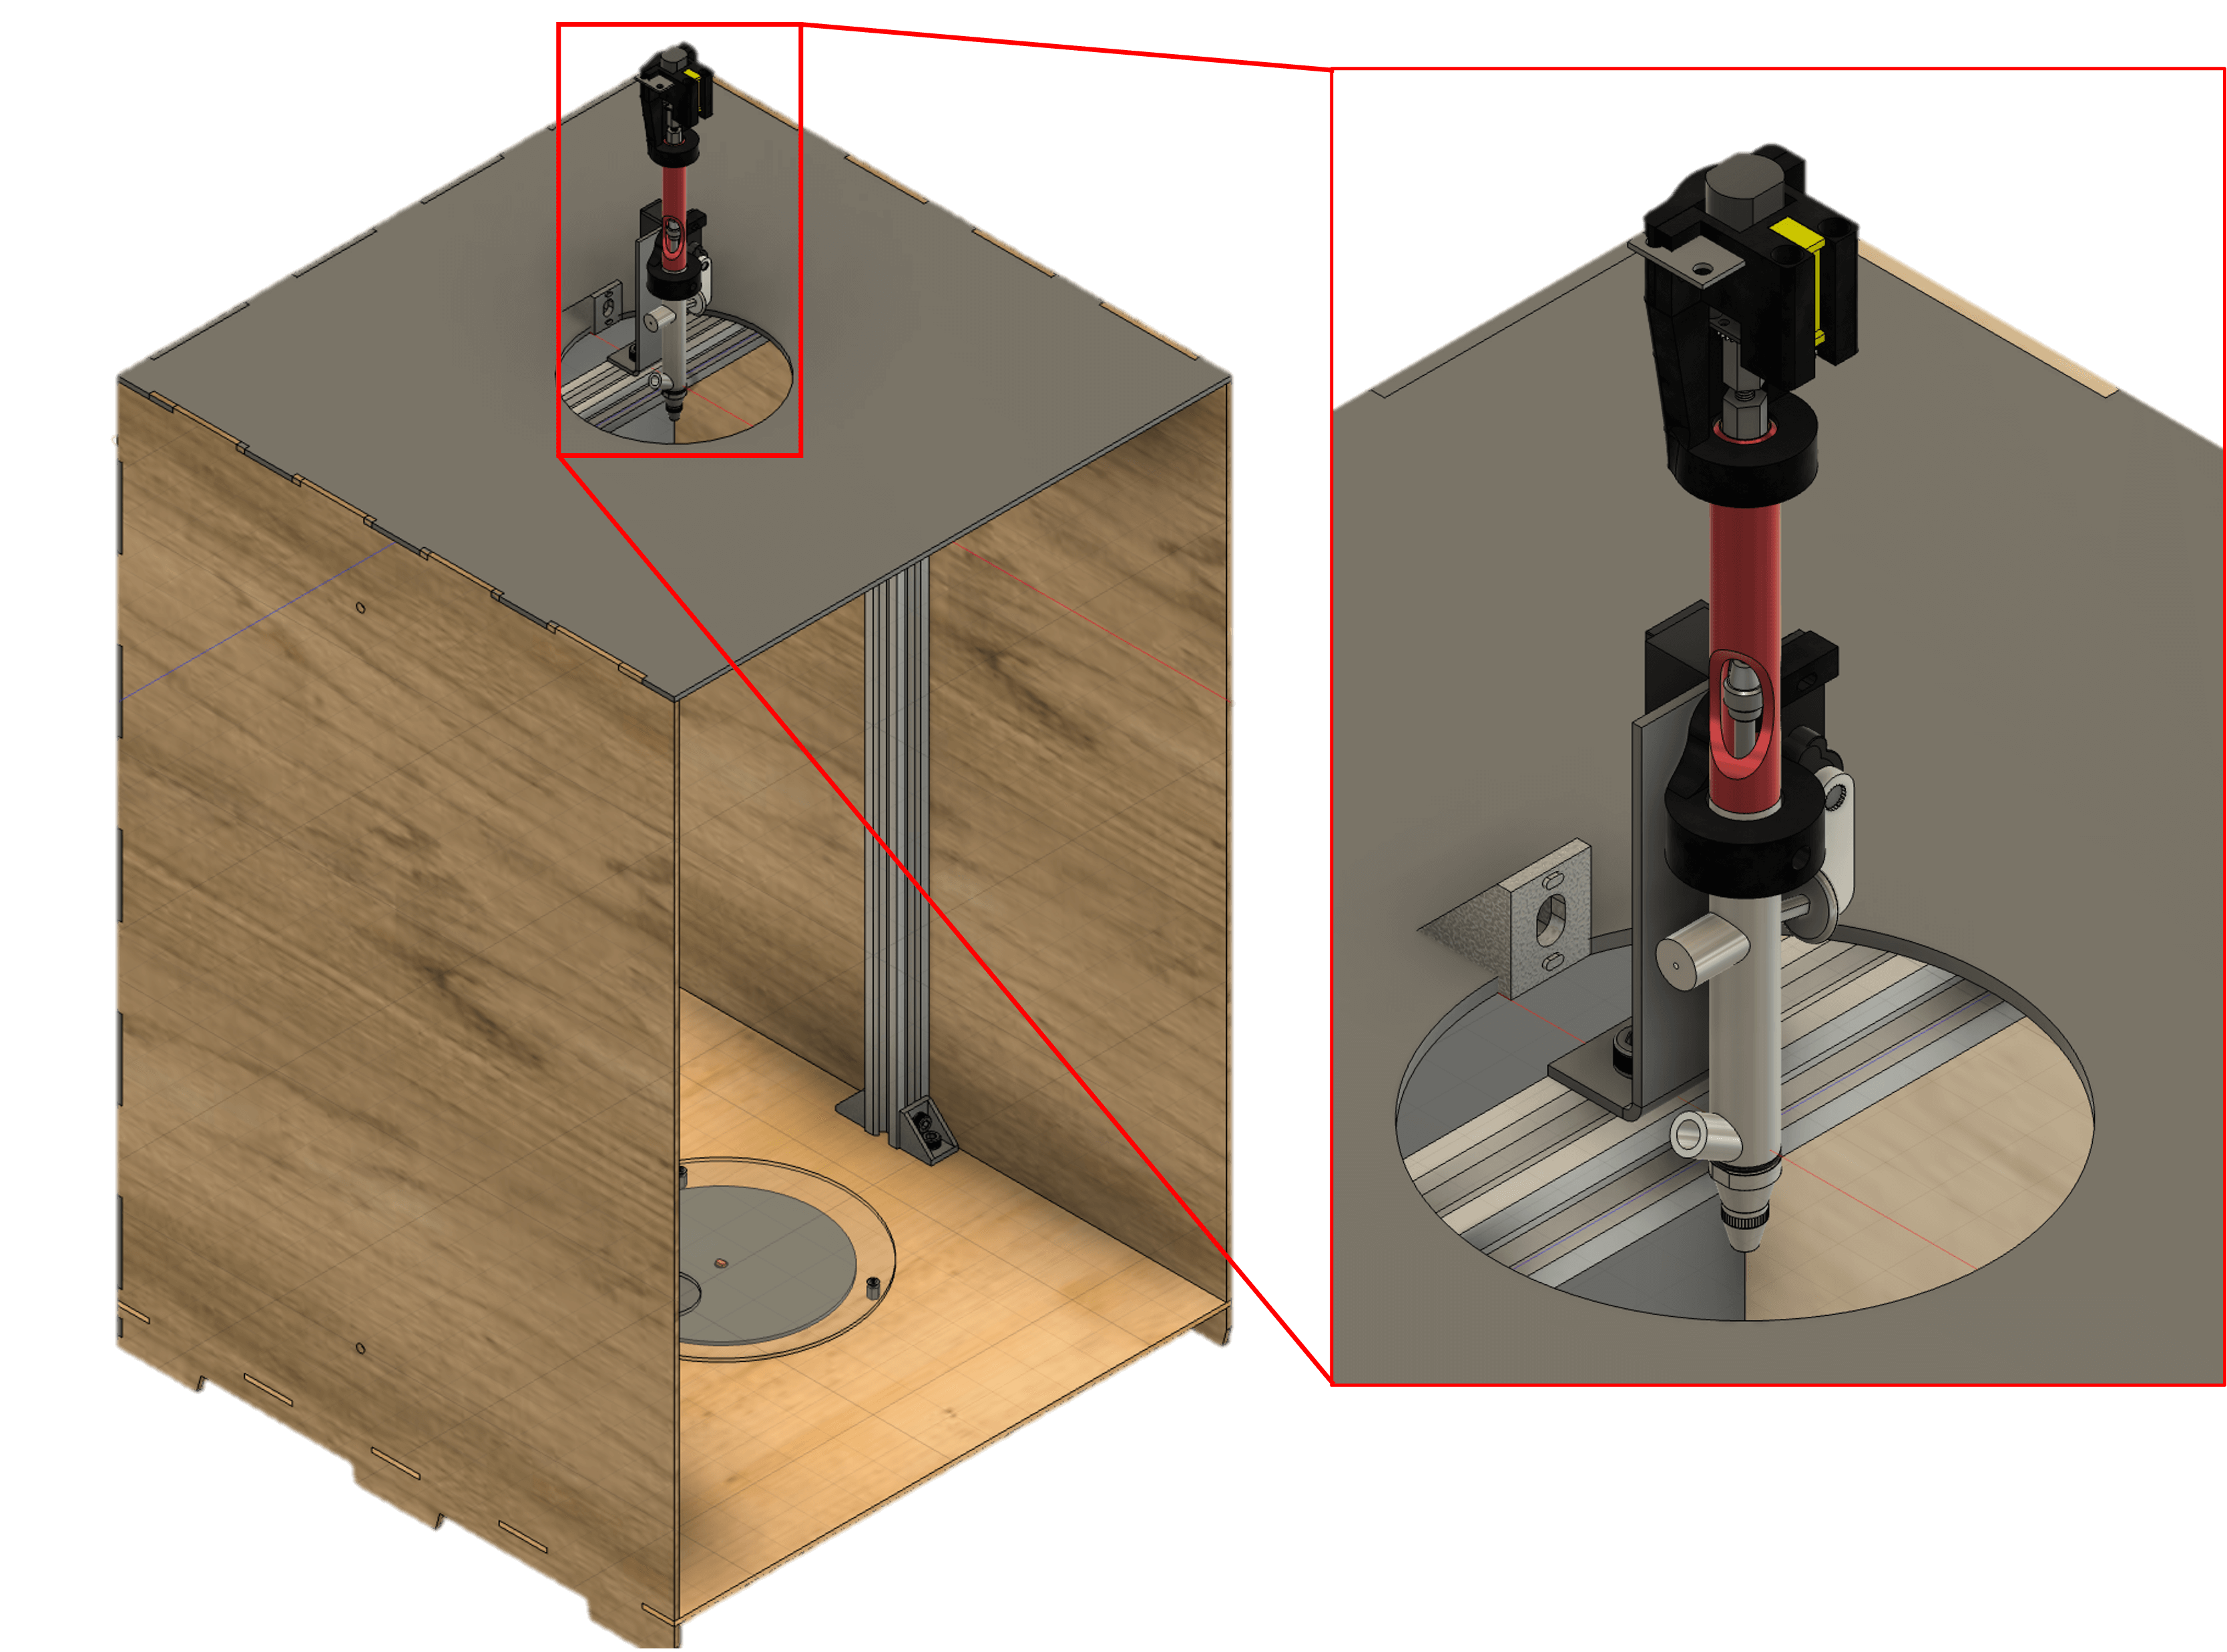
\includegraphics[width = \textwidth]{assets/figures/situation_initiale/machine_initiale.png}
  \caption[Machine originelle]{Machine originelle, avec un zoom sur le système de projection}
  \label{fig:Machine_originale}
\end{figure}

\newpage
La machine de projection se basait sur un aérographe robotisé, où des moteurs géraient les parties mobiles
de l'aérographe qui seraient normalement actionnée à la main :
\begin{figure}[H]
  \centering
  \begin{subfigure}{.35\textwidth}
    \centering
    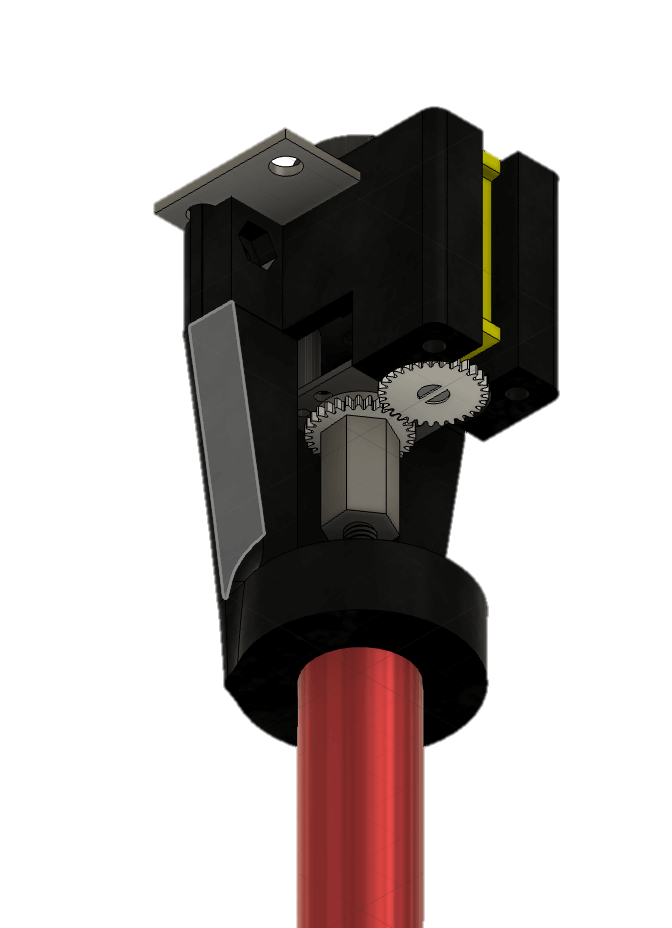
\includegraphics[width=1\linewidth]{assets/figures/situation_initiale/robotisation_aiguille.png}
    \caption{Robotisation de la position de l'aiguille}
    \label{fig:robot_aiguille}
  \end{subfigure}%
  \begin{subfigure}{.65\textwidth}
    \centering
    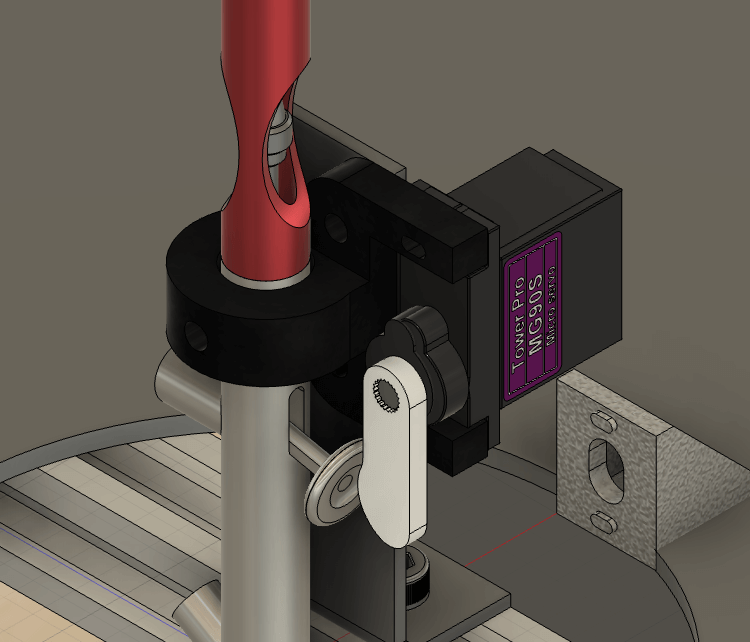
\includegraphics[width=.75\linewidth]{assets/figures/situation_initiale/Robotisation_projection.png}
    \caption{Robotisation du button d'activation du spray}
    \label{fig:robot_spray}
  \end{subfigure}
  \caption{Différentes robotisations de la machine originale}
  \label{fig:robotisations_aerographe}
\end{figure}

Un moteur pas-à-pas de type \textbf{28byj-48}, est situé en bas de l'appareil, ce dernier sert à faire tourner l'écran sur lui même,
c'est donc aussi où l'écran sera disposé lors de sa fabrication:
\begin{figure}[H]
  \centering
  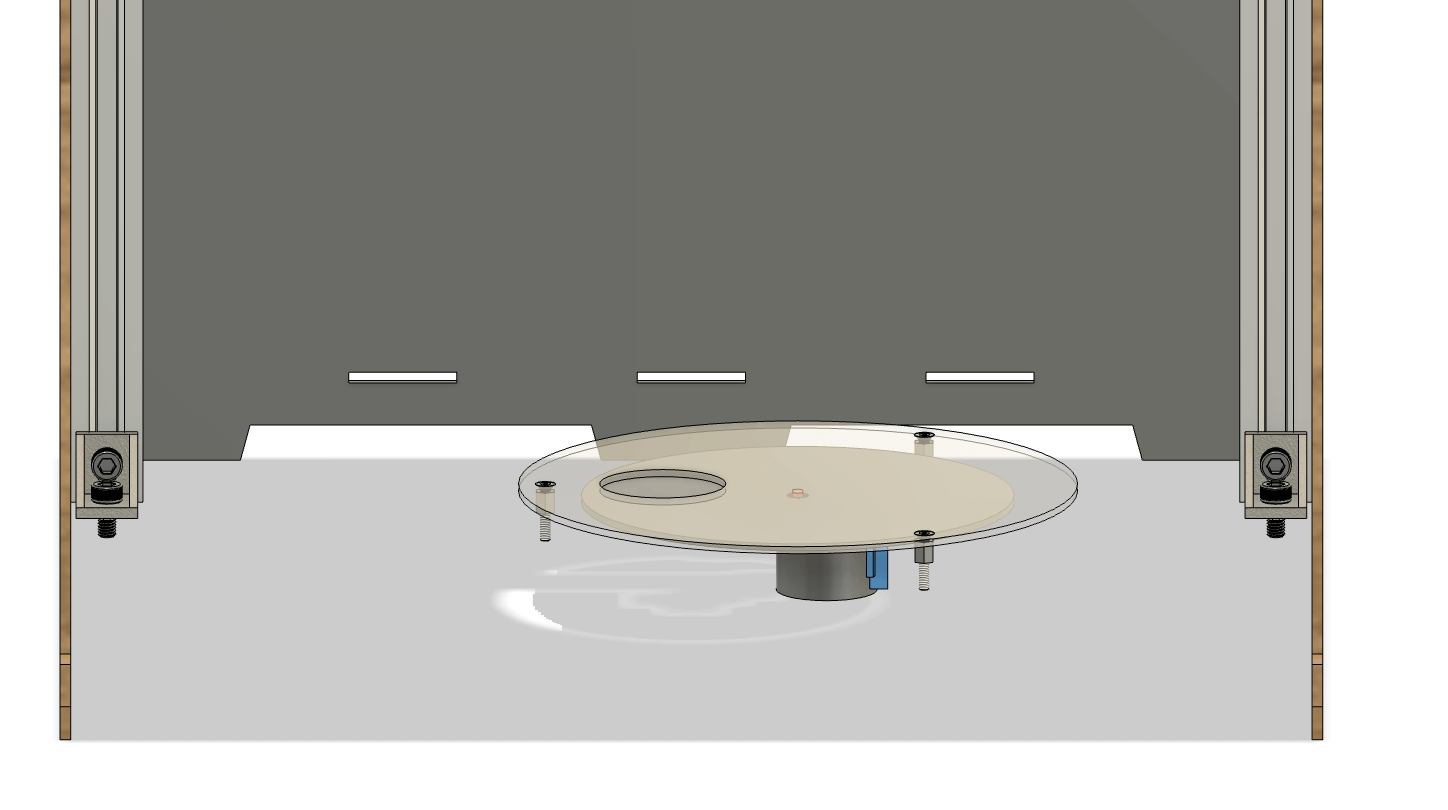
\includegraphics[width = \textwidth]{assets/figures/situation_initiale/rotation_ecran_initiale.png}
  \caption[Rotation écran initiale]{Système de rotation de l'écran}

\end{figure}

\newpage
Tout ces éléments sont contrôlés par un PCB et un arduino nano :
\begin{figure}[H]
  \centering
  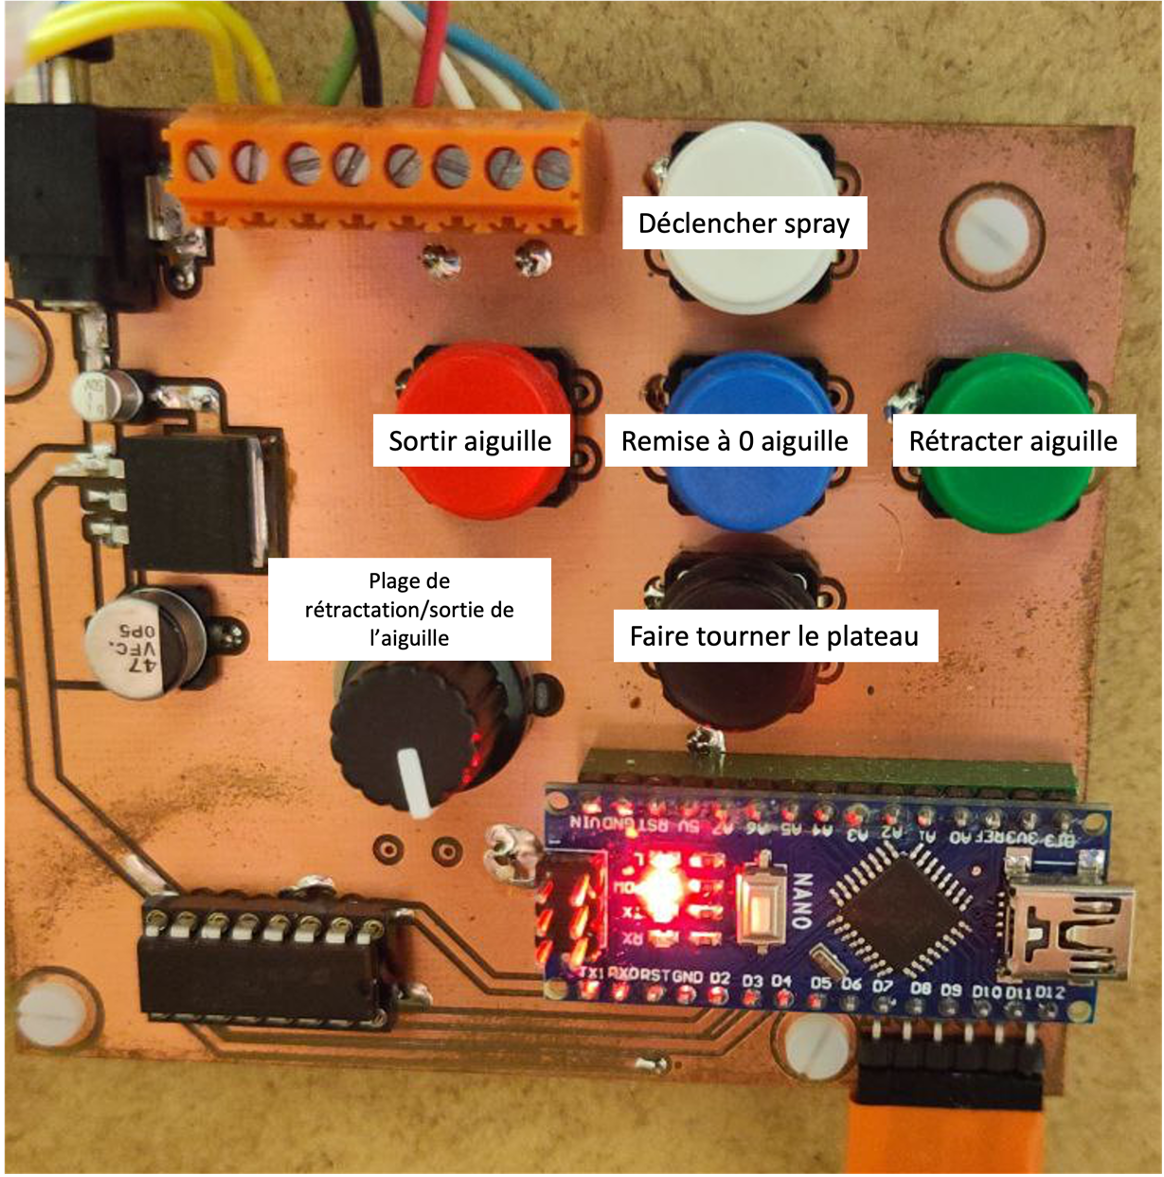
\includegraphics[width = 0.8\textwidth]{assets/figures/situation_initiale/PCB_machine_originale.png}
  \caption[PCB machine initiale]{PCB de la machine initiale et légende de chaque boutons}\label{PCB_machine_initial}
\end{figure}

\newpage
\section{Problèmes avec la machine}
En effet, la machine d'origine présente plusieurs inconvénients.
\subsection{Aérographe}
\subsubsection{Motorisation}
Comme montré dans la \autoref{fig:robotisations_aerographe}, l'aérographe est robotisé avec un moteur DC pour contrôler l'aiguille et un servo moteur pour activer
ou désactiver la projection de liquide. Ces deux éléments sont capricieux, le moteur DC de l'aiguille est relié à un encodeur (pour calculer la position de l'aiguille) à l'aide de deux petits engrenages en
plastique, ces engrenanges en plastiques étant tout petits ils se sont usés, en plus de cela l'encodeur est monté seulement par compression sur le support du moteur, donc au fil des utilisations, les efforts
normaux des engrenages repoussent l'encodeur, le moteur ne sait donc plus où il se trouve et se met à tourner indéfiniment.

De plus la pièce qui tient le moteur et qui se fixe sur l'aérographe n'exerce pas assez de pression sur ce dernier, si l'aiguille résiste lors de son mouvement
la pièce de support se délogera de son emplacement :

\begin{figure}[H]
  \centering
  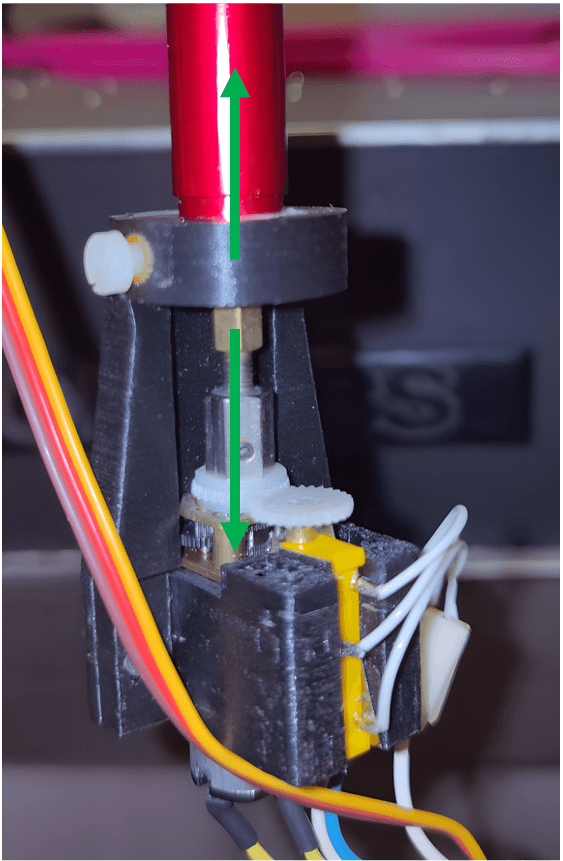
\includegraphics[width = 0.5\textwidth]{assets/figures/situation_initiale/moteur_desolidarisation_aerographe.png}
  \caption{Support moteur désolidarisé}
\end{figure}


\newpage
\subsubsection{État général}
Concernant l'état général de l'aérographe, ce dernier n'est pas idéal.
Le joint de la tête de projection est en bout de vie, il fuit et fait des bulles lors de l'utilisation de la machine:
\begin{figure}[H]
  \centering
  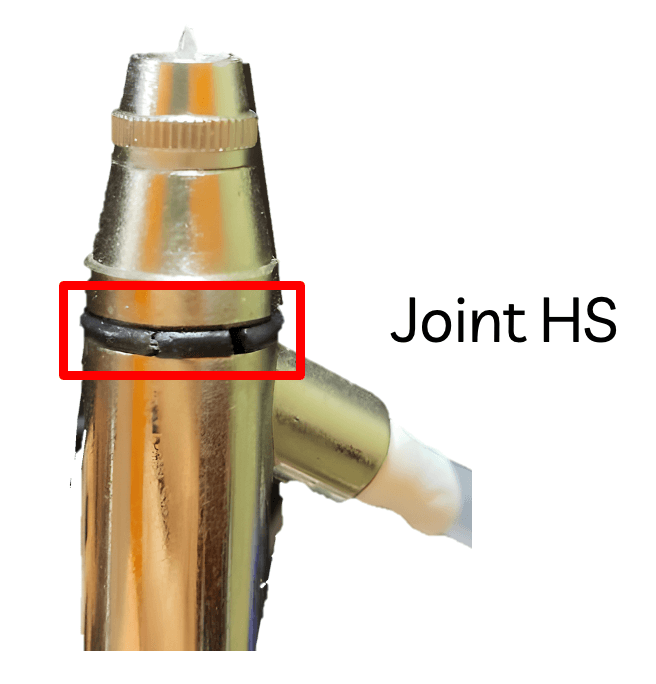
\includegraphics[width = 0.5\textwidth]{assets/figures/situation_initiale/joint_aerographe_HS.png}
  \caption{Joint sec et craquelé}
\end{figure}

Le support de l'aérographe qui permet de maintenir ce dernier sur le profilé alu du caisson de la machine est craqué,
ce dernier ne remplis plus sa fonction, l'aérographe bouge dans tout les sens et tourne sur lui-même :
\begin{figure}[H]
  \centering
  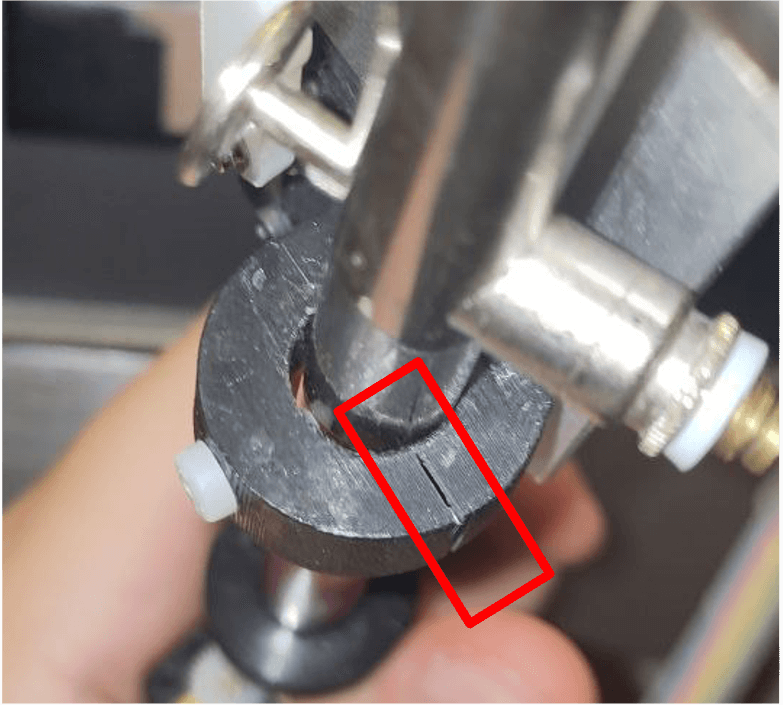
\includegraphics[width = 0.5\textwidth]{assets/figures/situation_initiale/support_aerographe_casse.png}
  \caption{Support aérographe cassé}
\end{figure}